\begin{center}
\Huge
Grafer for potensfunktioner
\end{center}

\section*{Potensfunktioner}
\stepcounter{section}

Vi vil nu betragte grafer for potensfunktioner. Vi skal mere præcist se, hvad tallene $a$ og $b$ har af betydning for grafen for en potensfunktion $f$ givet ved
\begin{align*}
	f(x) = b\cdot x^a.
\end{align*}

Grafer for potensfunktioner falder ind i én af tre klasser; aftagende potensfunktioner, voksende potensfunktioner, der vokser mere og mere og voksende potensfunktioner, der vokser langsommere og langsommere. Disse tre tilfælde kan ses på Figur \ref{fig:tregrafer}.
\begin{figure}[H]
	\centering
	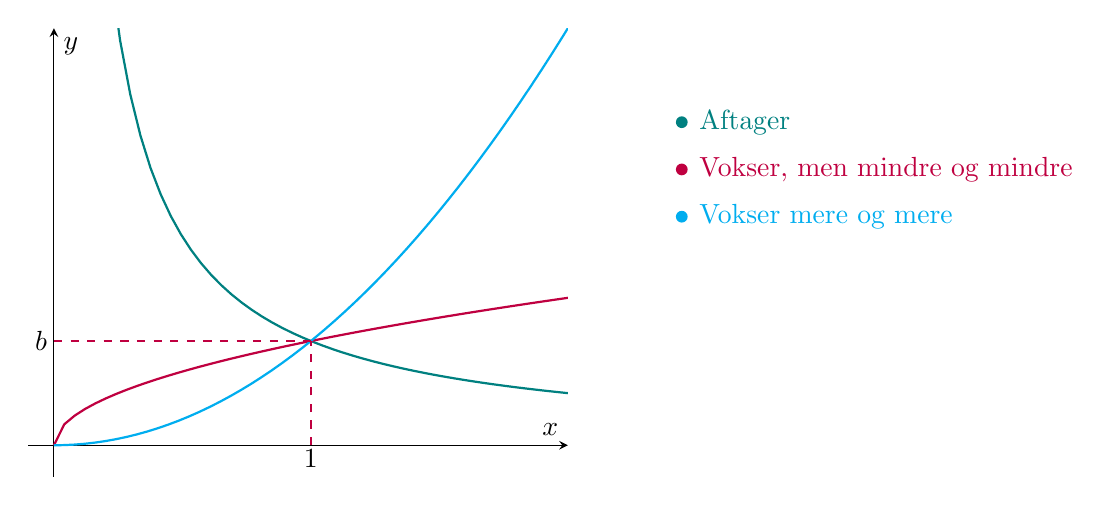
\begin{tikzpicture}
		\begin{axis}
			[axis lines = center,
			xmin = -0.1, xmax = 2,
			ymin = -0.3, ymax = 4,
			ticks = none,
			xlabel = $x$, ylabel = $y$]
			\addplot[thick, color = teal, samples = 100, domain = 0.1:4] {1/x};
			\addplot[thick, color = purple, samples = 100, domain = 0:4] {x^0.5};
			\addplot[thick, color = cyan, samples = 100, domain = 0:4] {x^2};
			\draw[thick, color = purple, dashed] (axis cs:1,0) -- (axis cs:1,1);
			\draw[thick, color = purple, dashed] (axis cs:0,1) -- (axis cs:1,1);
			\node at (axis cs:-0.05,1) {$b$}; 
			\node at (axis cs:1,-0.13) {1};
		\end{axis}
		\node[color = teal, anchor = west] at (8.4,4+0.5) {Aftager};
		\node[color = purple, anchor = west] at (8.4,3.4+0.5) {Vokser, men mindre og mindre};
		\node[color = cyan, anchor = west] at (8.4,2.8+0.5) {Vokser mere og mere};
		\node[circle, fill, inner sep = 1.5pt, color = teal] at (8.3,4+0.5) {};
		\node[circle, fill, inner sep = 1.5pt, color = purple] at (8.3,3.4+0.5) {};
		\node[circle, fill, inner sep = 1.5pt, color = cyan] at (8.3,2.8+0.5) {};
	\end{tikzpicture}
	\caption{Tre typer af potensfunktioner}.
	\label{fig:tregrafer}
\end{figure}

I Opgave 1 skal I selv afgøre, hvordan $a$ og $b$ påvirker grafen for potensfunktionen $f$. 


\subsection*{Opgave 1}
I Maple-filen \textit{PotensgrafMedSkyder} på Lectio finder i en interaktiv potensfunktion, hvor I kan ændre på $a$ og $b$ for at se, hvad dette gør ved grafen for potensfunktionen. Filen findes også \href{https://raw.githubusercontent.com/ChristianJLex/TeachingNotes/master/2023-2024/Moduler1m/V%C3%A6kst_diverse/PotensgrafMedSkyder.mw}{\color{blue!60} her}, men så skal du alt efter din browser formentlig gemme filen først. Husk at gemme den som en .mw-fil.
\begin{enumerate}[label=\roman*)]
	\item Hvad skal der gælde for $a$ for at potensfunktionen er aftagende?
	\item Hvad skal der gælde for $a$ for at potensfunktionen er voksende, men mindre og mindre?
	\item Hvad skal der gælde for $a$ for at potensfunktionen er mere og mere voksende?
	\item Kan I gennemskue, hvordan man aflæser $b$-værdien. Brug eventuelt Figur \ref{fig:tregrafer} til hjælp.
\end{enumerate} 

\subsection*{Opgave 2}
Tre potensfunktioner $f$, $g$ og $h$ er givet ved
\begin{align*}
	f(x) &= 3\cdot x ^2\\
	g(x) &= 5\cdot x^{0.7}\\
	h(x) &= 4\cdot x^{-0.8}\\
\end{align*}
Deres grafer er givet på Figur \ref{fig:potensgrafer}.
\begin{figure}[H]
	\centering
	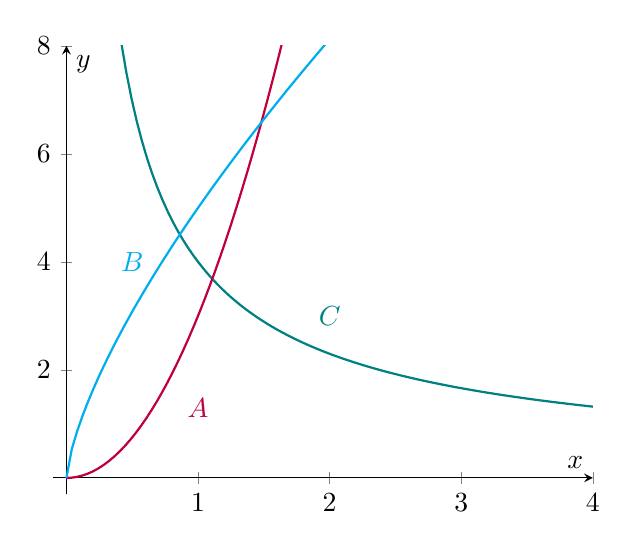
\begin{tikzpicture}
		\begin{axis}
			[axis lines = center, 
			xmin = -0.1, xmax = 4, 
			ymin = -0.3, ymax = 8,
			xlabel = $x$, ylabel = $y$]
			\addplot[color = teal, thick, domain = 0.1:4, samples = 100] {4*x^(-0.8)};
			\addplot[color = purple, thick, domain = 0.0:4, samples = 100] {3*x^(2)};
			\addplot[color = cyan, thick, domain = 0.0:4, samples = 100] {5*x^(0.7)};
			\node[color = purple] at (axis cs: 1,1.3) {$A$};
			\node[color = cyan] at (axis cs: 0.5,4) {$B$};
			\node[color = teal] at (axis cs: 2,3) {$C$};
		\end{axis}
	\end{tikzpicture}
	\caption{Graferne for de tre potensfunktioner $f$, $g$ og $h$.}
	\label{fig:potensgrafer}
\end{figure}

\begin{enumerate}[label=\roman*)]
	\item Afgør hvilke af graferne $A$, $B$ og $C$ der passer med funktionerne $f$, $g$ og $h$.
	\item Bestem $g(2)$ og brug Figur \ref{fig:potensgrafer} til at afgøre, om dette kan passe.
	\item Bestem skæringspunktet mellem graferne $A$ og $B$ ved at bruge deres forskrifter.
\end{enumerate}

\subsection*{Opgave 3}

\begin{enumerate}[label=\roman*)]
\item En cylinder har samme diameter som højde. Bestem den potensfunktion, der beskriver rumfanget af cylinderen som funktion af cylinderens radius. 
\item En kasse har bredde, højde og længde $x$. Bestem rumfanget af $x$, og afgør, hvad $a$ og $b$ er i denne potensfunktion.
\item For et bestemt objekt kan vindmodstanden på objektet beskrives ved 
\begin{align*}
F(v)= \frac{1}{2}v^2,
\end{align*}
hvor $v$ er hastigheden i $m/s$, objektet bevæger sig med, og $F$ er vindmodstanden målt i $N$. Hvad er vindmodstanden, når objektet bevæger sig med 50$m/s$? Hvor hurtigt skal objektet bevæge sig, for at modstanden på objektet er 20$N$?
\end{enumerate}
        